% 2011 年天津卷理科第 17 题：三棱柱 ABC-A1B1C1，H 为正方形 AA1B1B 的中心，C1H⊥平面 AA1B1B。
% 来源 PDF：普通高考/2011/2011天津理.pdf，SHA-256 4d77f7437f1f7191d1fd3cd766c7c3014859dec8fdd7a4d8f4bca348c0ef06e5。
% 原页：第 2 页（A3 三栏）第 1 栏上部，书页码 706。
% 重绘依据：照原页——AA1B1B 画成平行四边形（实为正方形），A、A1 在前下，B、B1 在后；
%   可见面为 ACC1A1 与 A1B1C1，B 为被遮挡的顶点；虚线为 AB、BC、BB1 三条被遮挡的棱及高 C1H；
%   H 标在正方形中心（对角线的交点）处。
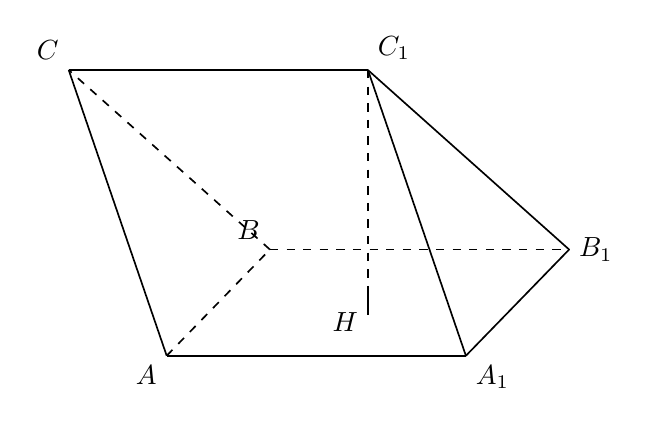
\begin{tikzpicture}[scale=0.95, >=stealth, semithick]
  \coordinate (A)  at (0,0);
  \coordinate (A1) at (4,0);
  \coordinate (B)  at (1.38,1.42);
  \coordinate (B1) at (5.38,1.42);
  \coordinate (H)  at (2.69,0.71);
  \coordinate (C1) at (2.69,3.82);
  \coordinate (C)  at (-1.31,3.82);

  % 可见棱（实线）
  \draw (C) -- (C1);     % 上棱 CC1
  \draw (C) -- (A);      % 棱 AC
  \draw (A) -- (A1);     % 底棱 AA1
  \draw (A1) -- (C1);    % 棱 A1C1
  \draw (C1) -- (B1);    % 棱 C1B1
  \draw (B1) -- (A1);    % 棱 A1B1

  % 被遮挡的棱与高（虚线）
  \draw[dashed] (A) -- (B);
  \draw[dashed] (B) -- (C);
  \draw[dashed] (B) -- (B1);
  \draw[dashed] (C1) -- (H);

  % H 处的垂足标记
  \draw ([yshift=-0.16cm]H) -- ([yshift=0.16cm]H);

  \node at (C) [above left] {$C$};
  \node at (C1) [above right] {$C_1$};
  \node at (B) [above left] {$B$};
  \node at (B1) [right] {$B_1$};
  \node at (A) [below left] {$A$};
  \node at (A1) [below right] {$A_1$};
  \node at (H) [below left] {$H$};
\end{tikzpicture}
